%!TEX root = ../zeeman.tex
Согласно квантовой теории излучения энергия атома $E$ может принимать лишь дискретные строго определенные значения. Совокупность таких разрешенных значений (уровней энергии) называют \textbf{энергетическим спектром атома}. Энергетический спектр атома может быть задан с помощью вполне определенного набора внутренних характеристик атома - его \textbf{квантовых чисел}. Наиболее точный смысл каждого квантового числа выясняется при решении \textbf{уравнения Шредингера}, в котором квантовые числа определяют \textbf{спектр собственных значений}. Мы же введем лишь названия и обозначения, а там, где это возможно, дадим краткую, более или менее наглядную и нс слишком строгую, характеристику квантовых чисел атома:

$n$ -- \textbf{главное квантовое число}, определяющее среднее расстояние электронного облака от ядра;

$L$ -- \textbf{орбитальное квантовое число}, характеризующее сумму моментов импульса электронов $\vec{P_L}$, связанных с их вращением вокруг ядра;

$S$ -- \textbf{спиновое квантовое число}, описывающее сумму собственных моментов импульса электронов $\vec{P_S}$, не связанных с их вращением вокруг ядра\footnote{Наличие собственною механического момента (спина) и магнитного момента у покоящегося электрона не имеет удовлетворительного наглядного толкования и должно восприниматься как факт, однозначно следующий из результатов многочисленных экспериментов.};

$J$ -- \textbf{азимутальное квантовое число}, которому ставится в соответствие полный механический момент электронов в атоме:

\begin{equation}
	\vec{P_J}=\vec{P_L}+\vec{P_S}
	\label{eq:1}
\end{equation}

$M_J$ -- \textbf{магнитное квантовое число}, название которого связано с тем, что энергия атома зависит от $M_J$ лишь при наличии внешнего магнитного поля: $E(n,J,L,S,M_J)$. В отсутствии магнитного поля для всех допустимых значений $M_J$ энергия атома имеет одно и то же значение $E(n,J,L,S,M_J)$ -- в этом случае говорят, что имеет место \textbf{вырождение} (неоднозначность) состояния атома по квантовому числу $M_J$. Из элементарной физики известно, что в магнитном поле могут изменить свою энергию лишь системы, имеющие (или приобретающие) \textbf{магнитный момент} $\vec{\mu}$, причем изменение энергии равно:

\begin{equation}
	\delta E=-(\vec{\mu}\vec{H})=-\mu_HH.
	\label{eq:2}
\end{equation}

Из сказанного ясно, что квантовое число $M_J$ характеризует проекцию магнитного момента атома $\vec{\mu}$ на направление внешнего магнитного поля $\vec{H}$.

\begin{figure}[tb]
	\centering
	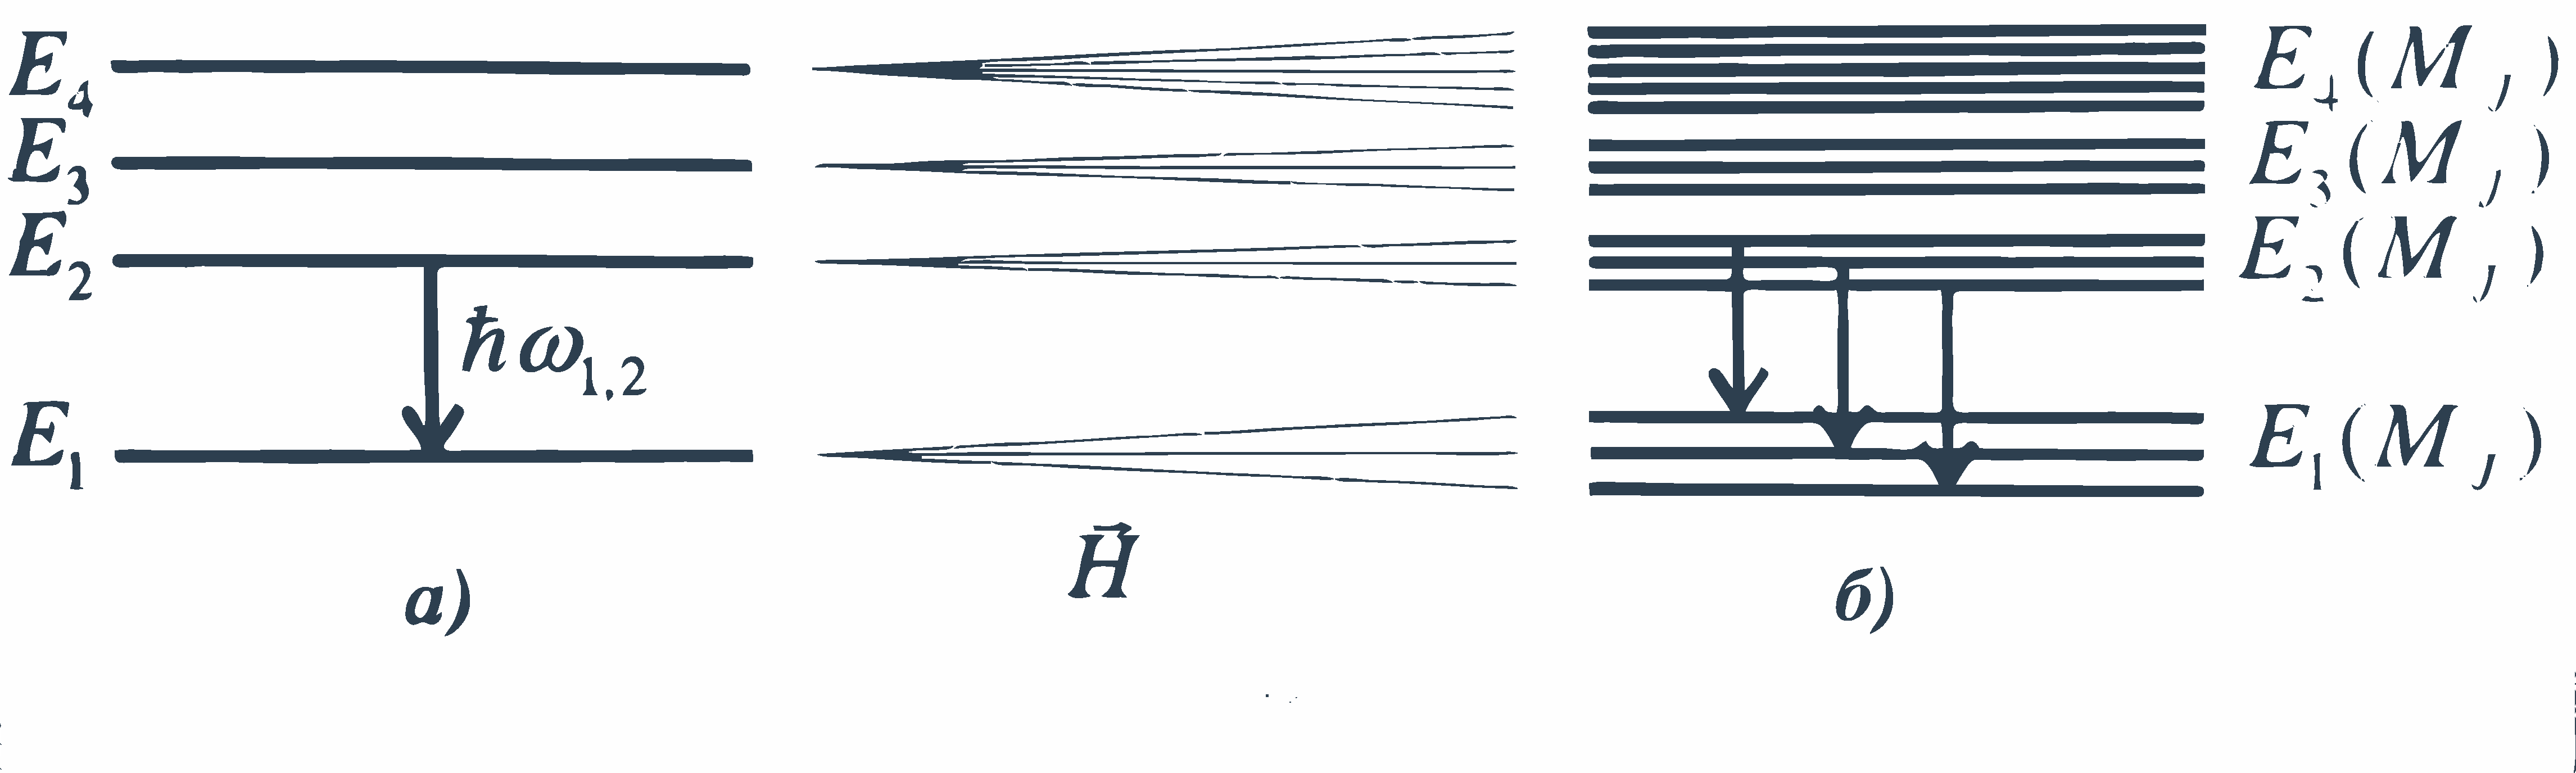
\includegraphics[width=\linewidth]{fig/fig1}
	\caption{Энергетическая структура атома и некоторые из возможных излучательных переходов
	а) в невозмущенном состоянии, б) при наложении внешнего магнитного поля}
	\label{fig:1}
\end{figure}

При переходе атома с более высокого энергетического уровня $E_2$ на более низкий $E_1$, излучается квант электромагнитной энергии (\ref{fig:1}) с частотой

\begin{equation}
\omega_{1,2}=\frac{E_2-E_1}{\hbar}
\label{eq:3}
\end{equation}
где $\hbar = 1.054\cdot10^{-27}$ эрг$\cdot$с -- постоянная Планка. Поскольку при наложении внешнего магнитного поля вырождение энергетических состояний $E_2$ и $E_1$ по квантовому числу $M_J$ снимается (т.е. происходит расщепление каждого энергетического уровня на несколько подуровней), в спектре излучения мы вместо одной наблюдаем несколько частот (линий) излучения (\ref{fig:1}). Этот эффект расщепления спектральных линий атомов в магнитном поле и называется \textbf{эффектом Зеемана}.
